\documentclass{article}
\usepackage[utf8]{inputenc}
\usepackage[english]{babel}
\usepackage{amsthm}
\usepackage{amssymb}
\usepackage{mathcomp}
\usepackage{amsmath}
\usepackage{natbib}
\usepackage{array}
\usepackage{wrapfig}
\usepackage{multirow}
\usepackage{tabularx}
\usepackage{graphicx}
\usepackage{geometry}
\usepackage{multicol}
\usepackage{blindtext}

\newtheorem{ishaan}{Theorem}[section]
\newtheorem{lemma}{Lemma}[section]
\renewcommand\qedsymbol{$\blacksquare$}

\title{Homework 3}
\author{Sean Eva}
\date{March 2022}

\begin{document}

\maketitle

\section{Theoretical Problems}
\begin{enumerate}
    \item [2. ]
    
    \begin{enumerate}
        \item 
        
        Since there are $n$ observations to sample from and there is an equal probability that any of the $n$ observations are selected. The probability the $j$th observation is selected as the first bootstrap observation is $\frac{1}{n}.$ Therefore, this implies that the probability that the $j$th observation is not the first bootstrap observation is $1-\frac{1}{n}.$
        
        \item
        
        Since bootstrap sampling is sampling with replacement, this is the same as before. The probability is still $1-\frac{1}{n}.$
        
        \item
        
        We will denote each bootstrapping sample as $S = \{s_1, s_2, ..., s_n\}$ for each $n$ bootstrapping samples. We already showed from the first two parts that $P(s_1\neq j) = P(s_2\neq j) = 1-\frac{1}{n}.$ Extending this same logic we know that $P(s_i \neq j) = 1-\frac{1}{n}$ for all $i \in \{1, 2, ..., n\}.$ Because each sample are independent, we are able to multiply the probabilities together and get, $P(s_1\neq j)\cap P(s_2\neq j) \cap ... \cap P(s_n\neq j) = \Pi_{i=1}^nP(s_i\neq j) = \Pi_{i=1}^n(1-\frac{1}{n}) = (1-\frac{1}{n})^n$ as desired.
        
        \item
        
        Since the formula above is not being in the set, we will instead use $1-(1-\frac{1}{n})^n$ and for $n=5$ we get $1-(1-\frac{1}{5})^5 = 0.672.$
        
        \item
        
        When $n=100$ we get $1-(1-\frac{1}{100})^{100} = 0.634.$
        
        \item
        
        When $n=10000$ we get $1-(1-\frac{1}{10000})^{10000} = 0.632.$
        
        \item
        
        The graphical representation of this is seemingly logarithmic. This is a visual representation of the $0.632$ rule in bootstrapping where we see that $\lim_{n\to \infty}1-(1-\frac{1}{n}0^n = 1-\frac{1}{e} \approx 0.632$.
        
        \item
        
        We created 10000 bootstrap samples from $\{1, 2, ..., 100\}$ and calculated what proportion of them contained the number $j = 4$. The simulation shows that this seems to happen with $63.5\%$ containing 4. This is reasonable because the more bootstraps we perform it will get close to $0.632$ or $63.2\%.$
        
    \end{enumerate}
    
    \item [1. ]
    
    \begin{enumerate}
        \item 
        
        From the question, we must find a cubic polynomial $f_1(x)$ with these properties.
        \begin{align*}
            f(x) &= \beta_0 + \beta_1x + \beta_2x^2 = \beta_3x^3 + \beta_4(x-\xi)_+^3\\
            &= \beta_0 + \beta_1x + \beta_2x^2 = \beta_3x^3\\
            &= a_1 + b_1x+c_1x^2+d_1x^3\\
            &= f_1(x).
        \end{align*} This matches the desired equation when $\beta_0 = a_1, \beta_1 = b_1, \beta_2 = c_1, \beta_3 = d_1$ and since $x\leq \xi$ we get that $(x-\xi)^3_+ = 0$.
        
        \item
        
        Consider, 
        \begin{align*}
            f(x) &= \beta_0 + \beta_1x + \beta_2x^2 + \beta_3x^3 + \beta_4(x-\xi)^3_+\\
            &= \beta_0 + \beta_1x + \beta_2x^2 + \beta_3x^3 + \beta_4(x-\xi)^3\\
            &= \beta_0 + \beta_1x + \beta_2x^2 + \beta_3x^3 + \beta_4(x^3 - 2\xi^2x + \xi^2x - \xi x^2 + 2\xi^2x - \xi^3)\\
            &= (\beta_0 -\beta_4\xi^3) + (\beta_1 + \beta_4\xi^2 + 2\beta_4\xi^2)x + (\beta_2-2\beta_4\xi-\beta_4\xi) x^2 + (\beta_3 + \beta_4)x^3\\
            &= a_2 + b_2x + c_2x^2 + d_2x^3\\
            &= f_2(x).
        \end{align*} This is true for $a_2 = \beta_0 -\beta_4\xi^3, b_2 = \beta_1 + \beta_4\xi^2 + 2\beta_4\xi^2, c_2 = \beta_2-2\beta_4\xi-\beta_4\xi, d_2 = \beta_3 + \beta_4.$
        
        \item 
        
        We have already shown that $f(x) = \beta_0 + \beta_1x + \beta_2x^2 + \beta_3x^3 + \beta_4(x-\xi)^3_+$ is a piecewise cubic polynomial that can be expressed in the form, $f(x) = \begin{cases}
        f_1(x) & \text{for } x \leq \xi\\
        f_2(x) & \text{for } x > \xi
        \end{cases}.$ At the knot $\xi$, we get: $f_1(\xi) = \beta_0 + \beta_1\xi + \beta_2\xi^2 + \beta_3\xi^3$ and $f_2(\xi) = \beta_0 + \beta_1\xi + \beta_2\xi^2 + \beta_3\xi^3$. This therefore, implies that $f_1(\xi) = f_2(\xi),$ so $f(x)$ is continuous at the knot $\xi.$
        
        \item
        
        If we consider the first derivatives $f_1'(\xi) = \beta_1 + 2\beta_2\xi + 3\beta_3\xi^2$ and $f_2'(\xi) = \beta_1 + 2\beta_2\xi + 3\beta_3\xi^2$. Therefore, we have that $f_1'(\xi) = f_2'(\xi)$ which implies then that $f'(x)$ is continuous at the knot $\xi.$
        
        \item
        
        If we consider the second derivatives, we get $f_1''(\xi) = 2\beta_2 + 6\beta_3\xi$ and $f_2''(\xi) = 2\beta_2 + 6\beta_3\xi.$ Similarly, since $f_1''(\xi) = f_2''(\xi)$ we have that $f''(x)$ is continuous at the knot $\xi.$
        
    \end{enumerate}
    
    \item [2. ]
    
    \begin{enumerate}
        \item 
        
        \begin{center}
        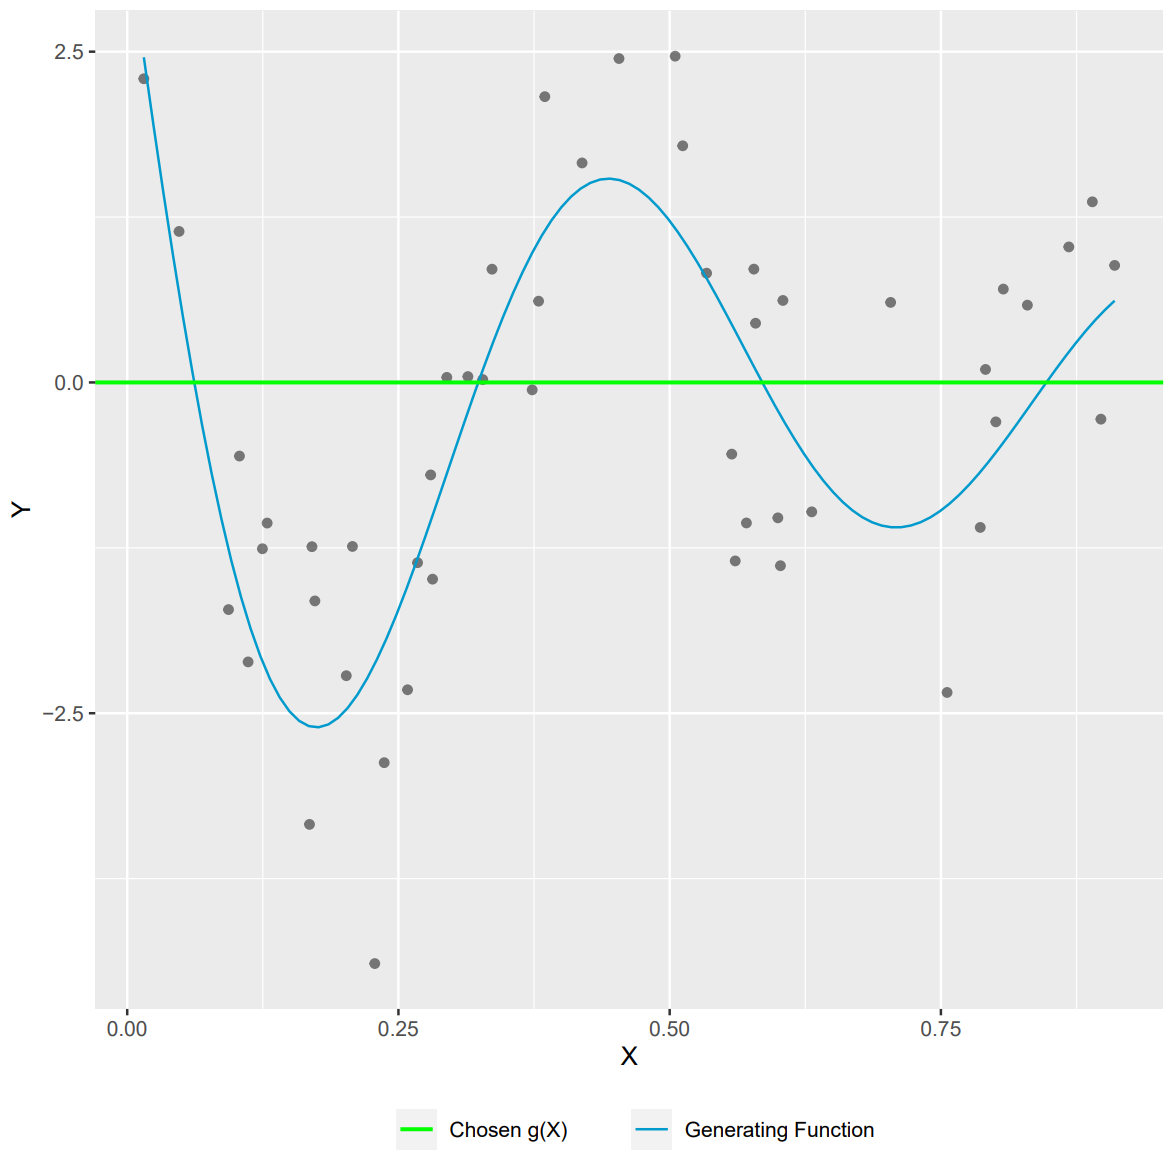
\includegraphics[width=8cm]{graph_2a.png}
        \end{center}
        
        \item 
        
        \begin{center}
        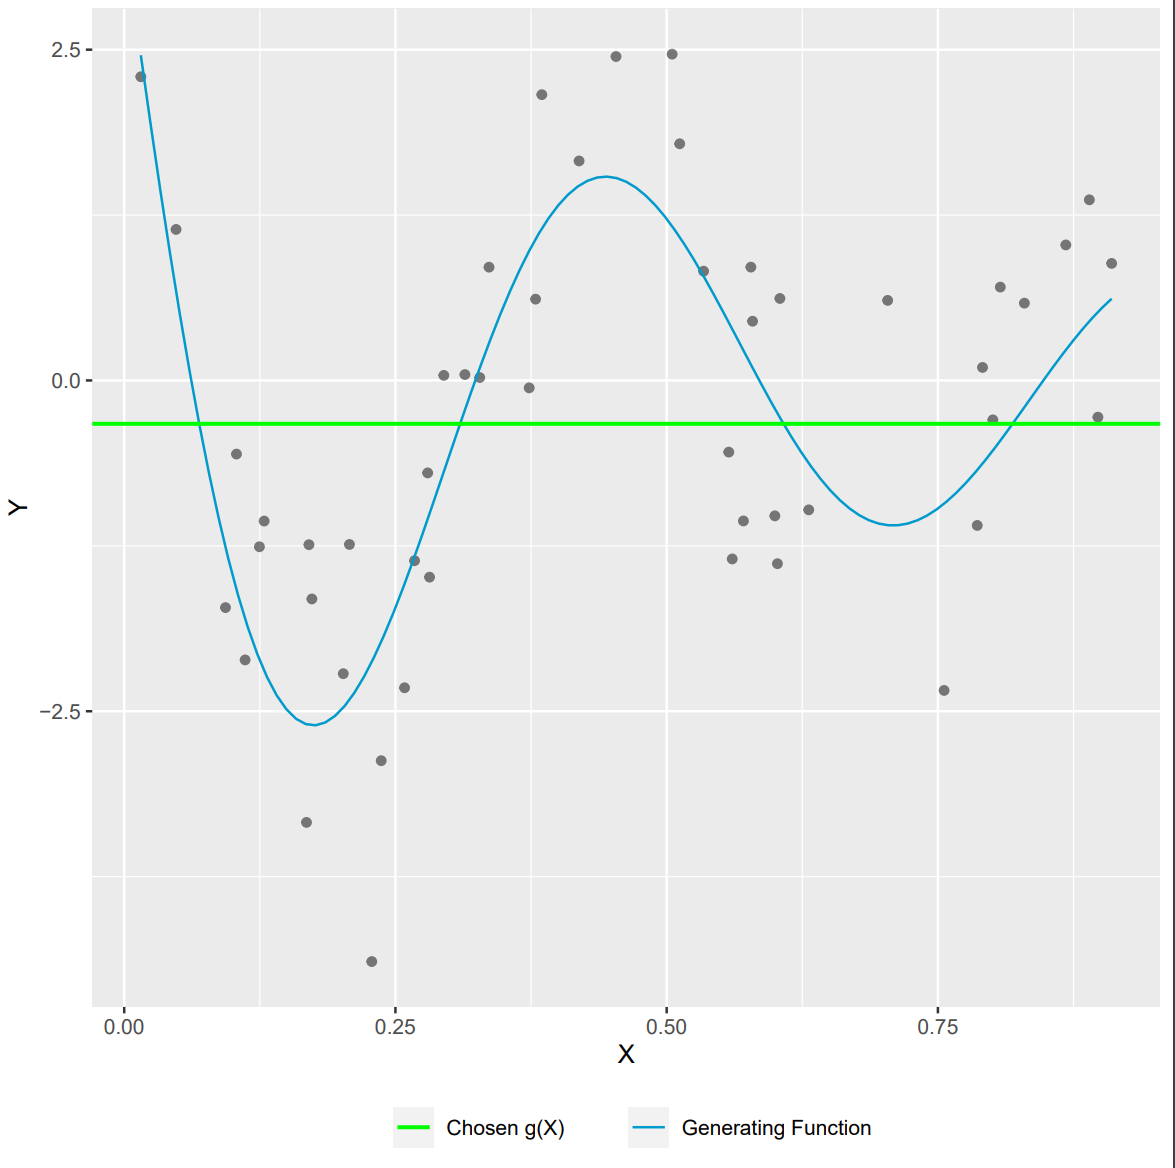
\includegraphics[width=8cm]{graph_2b.png}
        \end{center}
        
        \item 
        
        \begin{center}
        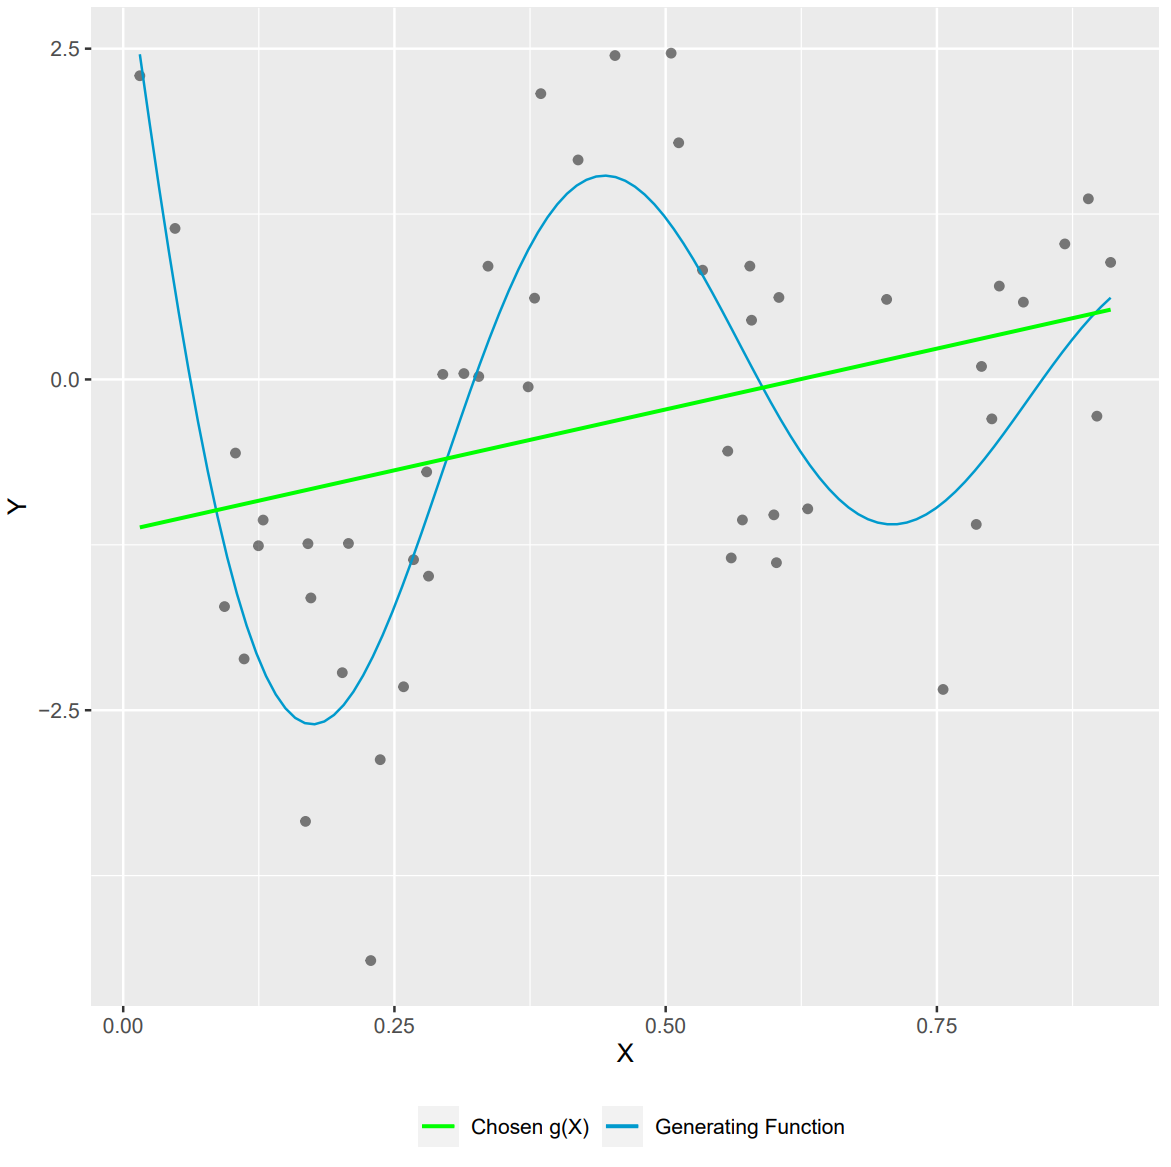
\includegraphics[width=8cm]{graph_2c.png}
        \end{center}
        
        \item 
        
        \begin{center}
        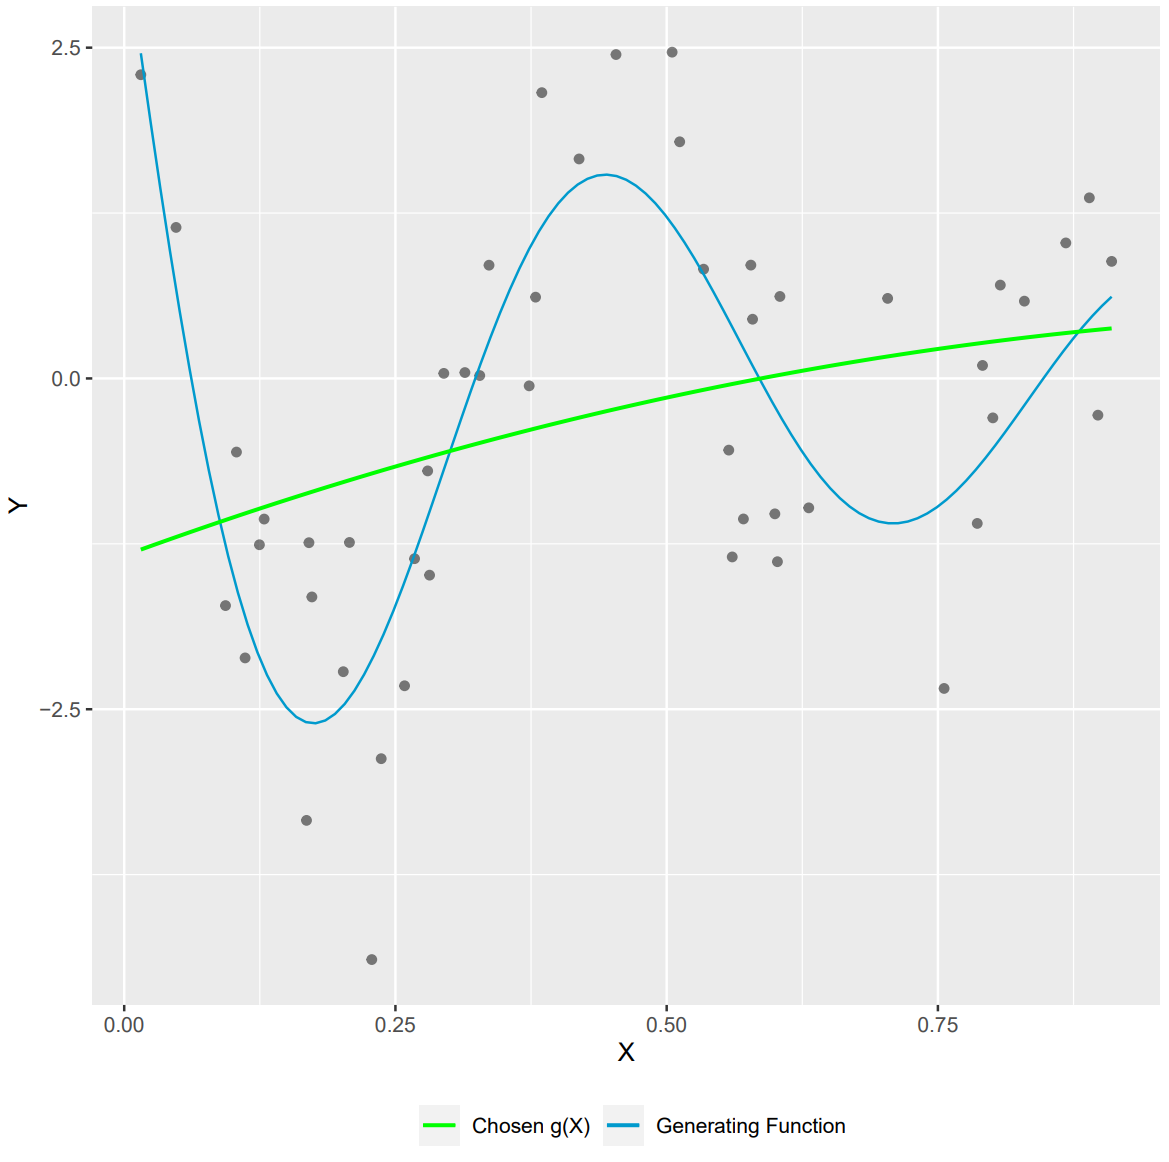
\includegraphics[width=8cm]{graph_2d.png}
        \end{center}
        
        \item 
        
        \begin{center}
        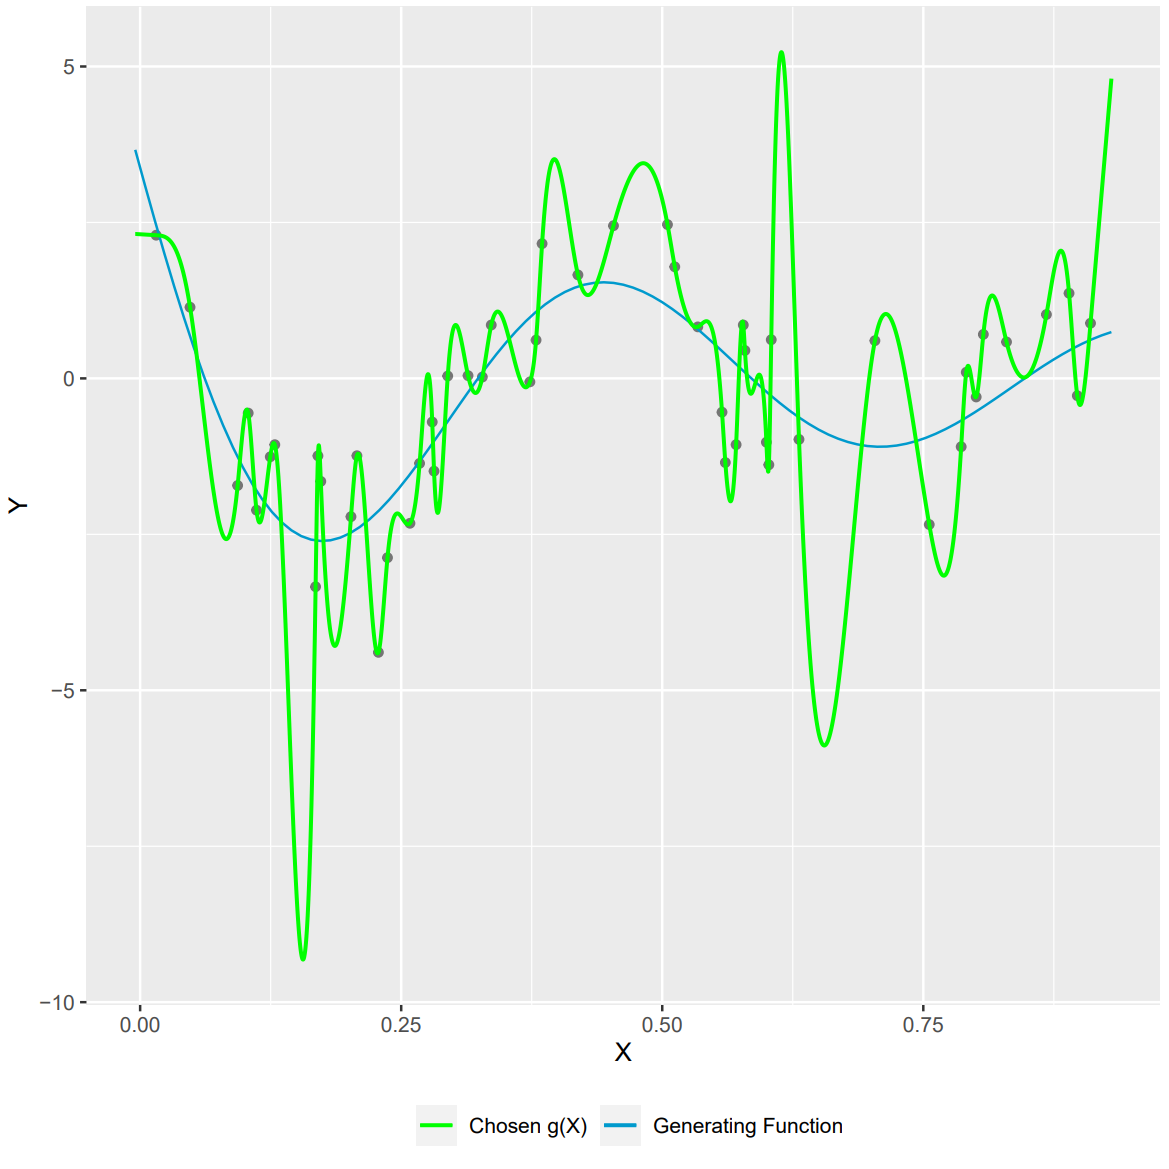
\includegraphics[width=8cm]{graph_2e.png}
        \end{center}
        
    \end{enumerate}
    
    \item [4. ]
    
    If we plug in these basis functions and coefficient estimates we get a fitted model. We are only interested in the model over the range $[-2, 6]$. For$X<0$ none of the indicator variables are true so $\hat{f}(X) = 1$ with a slope of $0.$ For $0\leq X < 1,$ the first indicator is true so $\hat{f}(X) = 1 + 1 = 2,$ so this is the intercept with a slope of $0.$ For $1\leq X\leq 2$, the first two indicator variables are true so we have $\hat{f}(X) = 1 + 1 - (X-1) * 1 = 3-X$, so the slope is $-1$ in this range. For $2\leq X\leq3$ none of the indicators are active again so we have a slope of $0$ with a value of $1.$ Then for $3 \leq X\leq 4$ we get $\hat{f}(X) = 3(X-3)$ so it has a slope of $3.$ Then on $4\leq x\leq 5$ we just get $\hat{f}(X) = 3$ with no slope. Lastly, $x > 5$ there is no indicator so we have a value of $1$ with no slope.\\
    \begin{center}
    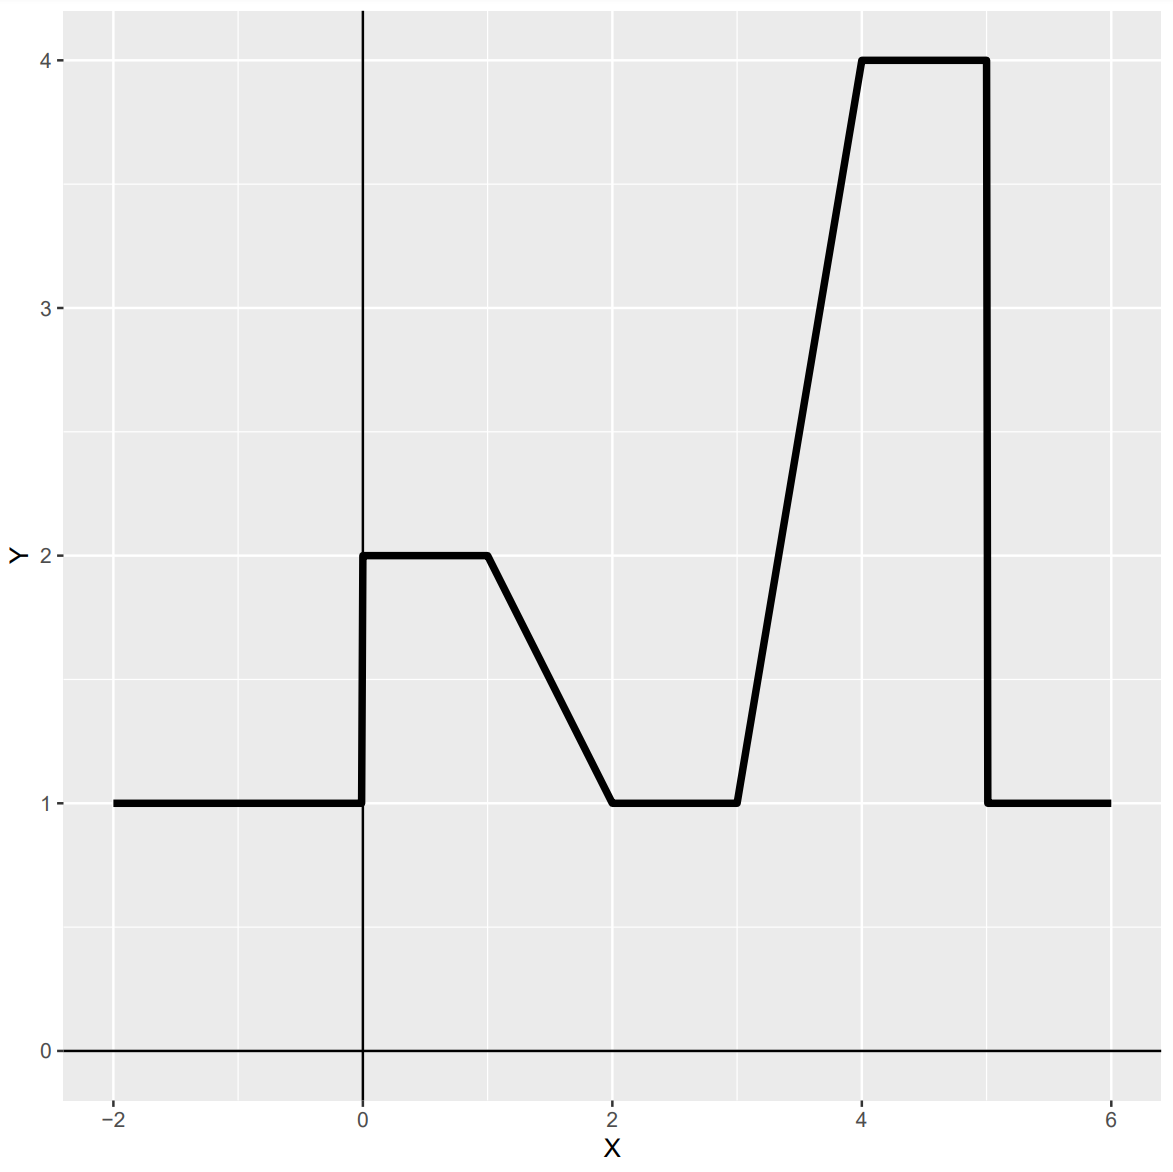
\includegraphics[width=10cm]{graph_4.png}
    \end{center}
    
    \item [5. ]
    
    \begin{enumerate}
        \item 
        
        Similar to question 2, as $\lambda$ increases, the penalty term will become more and more important in the equjation. For $\hat{g}_1, \lambda \to \infty$ makes $g^{(3)}(x)\to 0$. The higher order (most flexible) polynomial to satisfy this would be of the form $\hat{g}(x) = ax^2 + bx + c$ which would make the third derivative $0$. $\hat{g}_1$ will therefore be quadratic that minimizes the training RSS. For $\hat{g}_2, \lambda \to \infty$ makes $g^{(4)}(x)\to 0.$ The highest order (most flexible) polynomial to satisfy this would be of the form $\hat{g}(x) = ax^3 + bx^2 + cx + d$ which would make the fourth derivative 0. $\hat{g}_2$ will therefore be the cubic that minimizes the training RSS. Since $\hat{g}_2$ would be more flexible as the higher order polynomial, $\hat{g}_2$ would have the smaller training RSS.
        
        \item
        
        It depends whether the true relationship between $x$ and $y$ is better approximated with a cubic or quadratic relationship. It is possible that $\hat{g}_2$ could be overfitted and have a larger test RSS, or $\hat{g}_1$ could be underfit and have a larger test RSS.
        
        \item
        
        For $\lambda = 0$ there is nor restriction at all on $g(x)$, so both $\hat{g}_1$ and $\hat{g}_2$ would have the same training RSS (of zero is all the $x_i$ are unique). With no restriction at all on $g$ we can simply have any function that interpolates all the training observations (like question 2).
        
    \end{enumerate}
    
    \item [6. ]
    
    \begin{enumerate}
        \item 
    \end{enumerate}
    
\end{enumerate}
\section{Programming}
\begin{enumerate}
    \item [8. ]
    
    \begin{enumerate}
        \item 
        
        We have $n = 100$ and $p = 2.$ The model used to generate the data is: $Y = X - 2X^2 + \epsilon$ for $\epsilon ~ N(0, 1)$
        
        \item
        
        We have the underlying relationship: 
        \begin{align*}
            f(X) &= X-2X^2\\
            &= X(1-2X)\\
            f(X) = 0 &\Rightarrow X\in \{0, 0.5\}.
        \end{align*} And we have that $f''(0.25) = -4 < 0,$ so $0.25$ is a maximum. This means that since $\epsilon ~ N(0, 1)$ is centered at $0$, we should expect the data to show a quadratic relationship between $X$ and $Y,$ with a maximum at $\approx X = 0.25$, and crossing the x-axis at $\approx X = 0$ and $X = 0.5.$
        
        \item
        
        \begin{enumerate}
            \item 
            
            7.288
            
            \item
            
            0.937
            
            \item
            
            0.957
            
            \item
            
            0.954
            
        \end{enumerate}
        
        \item
        
        \begin{enumerate}
            \item 
            
            7.288
            
            \item
            
            0.937
            
            \item
            
            0.957
            
            \item
            
            0.954
        \end{enumerate}
        We get the results. This is because with LOOCV, there is no randomness, there can only be one LOOCV error statistic.
        
        \item
        
        The quadratic model has the smallest LOOCV error, although the second, third, and fourth order polynomials fits perform almost identically, This is as we would expect, from part a we know that the relationship between $X$ and $Y$ is defined as a second order polynomial of $X.$ This implies that the penalty of using a third and fourth order polynomial is greater than the benefit of using a second order polynomial. 
        
        \item
        
        There is no evidence at the 5\% level that the coefficients for $X^3$ and $X^4$ are non-zero. This is in agreement with the LOOCV error, which also concluded that there was no reason to select the third or fourth-order fits over the second order fit.
    \end{enumerate}
    
    \item [6. ]
    
    \begin{enumerate}
        \item 
        
        I iterated through polynomials of order 1 to 10 of age, using 10-fold cross-validation to select the best model. This result in the selection of the third-order polynomial.
        
        \item
        
        We cut age into 20 intervals for the step function, using cross-validation to select the best model. The selected model had 12 intervals of age. 
        
    \end{enumerate}
    
    \item [7. ]
    
    Year is the only other number variable in the dataset, and can only take 7 unique values between 2003 and 2009 so it doesn't seem appropriate to use splines to describe the relationship. Because of the discrete nature of year we will use a step function first. The step function between year and wage is vastly uninformative. For marital status it appears that married workers earn more. Due to the low values we are going to combine widowed with divorced to make something like previously married for modelling. In this dataset, asian men earned the most followed by white men and black men. You can potentially combine categories again for modelling. Using the region variable we see that we are only using mid-atlantic male workers so we can see an obvious split. the jobclass variable is very balanced. Most of the workers don't have health insurance; however, the employees with health insurance are on average paid more. 
    
    \item [9. ]
    
    \begin{enumerate}
        \item 
        
        The fit looks pretty good for this most part but we can see the limitations in the tails of dis.
        
        \item
        
        Cubic and quartic fits seem to be the most reliable. As we might expect, the training RSS decreases monotonically as flexibility increases so the minimum training RSS is for degree 10.
        
        \item
        
        If we use 10-fold cross-validation to provide an out-of-sample error estimate for polynomial regression from degrees 1 to 10. The selected model was of degree 3. The large instibility in the MSE estimate for higher-order polynomials is because of the significant flexbility in the fits. When we partition the data into 10 segments for cross-validation there will be considerable variability in the fitted model for higher values of dis. This result could change considerably if we exclude outliers which shows how high-variance the higher order polynomials are at the tails. 
        
        \item
        
        Since there are 4 degrees of freedom then the amount of knots is $K = 0$ since there are no other degrees of freedoms to be given to the knots. The cubic polynomials from the 4 degrees of freedom fit the data fairly well.
        
        \item
        
        When trained and tested on the data, a model with high complexity will be deemed the best.
        
        \item
        
        When validated on out-of-sample data a simpler model is chosen. Just like with the polynomial validation we can see that this is the most complex model that does not show obvious signs of overfitting.
        
    \end{enumerate}
    
\end{enumerate}
\end{document}
